\documentclass[12pt,a4,finnish,pdflatex%,handout
]{beamer}
\definecolor{MyGreen}{RGB}{50, 120, 50}
\usecolortheme[named=MyGreen]{structure}

\usepackage{babel}
\usepackage[utf8]{inputenc}
\usepackage[T1]{fontenc}
\usepackage{amsmath,amssymb} 
\usepackage{animate}
\usepackage{multimedia}

\usepackage{natbib}
\bibpunct[: ]{(}{)}{,}{}{}{;}

\usepackage{tikz}

\usepackage{tipa}

\usepackage{hyperref}

\setbeamertemplate{navigation symbols}{}

\graphicspath{{figures/}}

\setlength{\leftmargini}{0pt}
\setlength{\leftmarginii}{1em}

\newcommand{\kommentti}[1]{
  {\bf[#1]}
}



\begin{document}
\title{Ultraäänikuvauksen toimintaperiaate ja puheartikulaation mittaaminen\\
a.k.a. Ultraluento 1
} 
\author{Pertti Palo} 
\date{8. huhtikuuta 2024}

\frame{\titlepage
} 

\frame{\frametitle{Kuka tää tyyppi on?}
  \begin{columns}
    \begin{column}{5cm}
      \includegraphics[width=\columnwidth]{uti_eva.png}
    \end{column}
    \begin{column}{5cm}
      \begin{itemize}
      \item Pertti Palo
      \item Minulla on pari tutkintoa Otaniemestä ja viimeisimpänä
        fonetiikan tohtorin paperi.
      \item Puhun sujuvaa foneetikkoa ja insinööriä, ja tiedän paljon
        puheen mittaus- ja analyysimenetelmistä.
      \end{itemize}
    \end{column}
  \end{columns}
} 

\frame{\frametitle{Johdantoa: Millaisissa (ultraääni) projekteissa olen ollut mukana?}
  \begin{itemize}
  % \item Ultraäänellä on tutkittu kielen ja kurkunpään liikkeitä monella eri
  % tavallla ja ultraääntä on yhdistetty myös muihin mittausmenetelmiin --
  % esimerkiksi EMA, EEG, EGG ja erityisesti käytännössä aina audio.
  \item Itse olen keskittynyt puhe-eleiden ajoituksen tutkimiseen aloittaen
  puheen alun ilmiöistä ja sittemmin tarkastellut koko puhunnosta artikulaation
  alusta lihasten rentoutumiseen asti.
  \item Lisäksi olen annotoinut ja murskannut dataa mm.:
  \begin{itemize}
    \item Kitahalkion korjaamisen jälkeistä puheterapiadataa,
    \item Levantin arabiankielen faryngaaliäänteiden vertailudataa, ja
    \item Eri kielten koartikulaation vertailudataa.
  \end{itemize}
  \end{itemize}
}

\frame{\frametitle{Mitä tuleman pitää - yleisesti}
  \begin{itemize}
  \item 1. Luento: Ultraääni puheentutkimuksessa
    \begin{itemize}
    \item Puheartikulaation mittaaminen ultraäänellä
    \item Video ultraäänen käytöstä puheterapiassa
    \item Ultraäänikuvauksen toimintaperiaate ja käytännön ominaisuudet
    \end{itemize}
  \item {\usebeamercolor[gray]{} 2. Luento: Ultraäänikuvauksella tallennetun puhemateriaalin analyysi}
    \begin{itemize}
    \item {\usebeamercolor[gray]{} Esimerkkejä tutkimusprojekteista}
    \item {\usebeamercolor[gray]{} Analyysimenetelmien esittely}
    \item {\usebeamercolor[gray]{} Analyysiesimerkki}
    \end{itemize}
  \end{itemize}
}

\frame{\frametitle{Mitä tuleman pitää - tänään}
  \begin{itemize}
  \item Puheartikulaation mittaaminen ultraäänellä
    \begin{itemize}
    \item Yleistä
    \item Fyysinen toimintaperiaate
    \item Miltä kuva näyttää?
    \item Tallennussession vaiheet
    \end{itemize}
  \item {\usebeamercolor[gray]{} Video ultraäänen käytöstä puheterapiassa}
  \item {\usebeamercolor[gray]{} Ultraäänikuvauksen toimintaperiaate ja ominaisuudet} 
  \begin{itemize}
    \item {\usebeamercolor[gray]{} Etuja}
    \item {\usebeamercolor[gray]{} Rajoitteita: Menetelmä ja ihmiset}
    \item {\usebeamercolor[orange]{} \bf Kysellään}
    \end{itemize}
  \end{itemize}
}

\frame{
  \centering
  {
    \vfill
    \bf \Large 
    \usebeamercolor[fg]{title}
    Johdanto ultraäänikuvaukseen menetelmänä
    \vfill
  }
}

\frame{\frametitle{Yleistä I}
  \begin{itemize}
  \item Kasvavassa suosiossa puheentutkimuksen parissa.
  \item Puheterapiassa potentiaalisesti hyödyllinen paitsi välittömän
    palautteen annossa (osuiko liike oikeaan paikkaan) myös tuomassa
    terapeutille lisätietoa erityisesti piilovirheistä.
  \end{itemize}
  
  \centering
  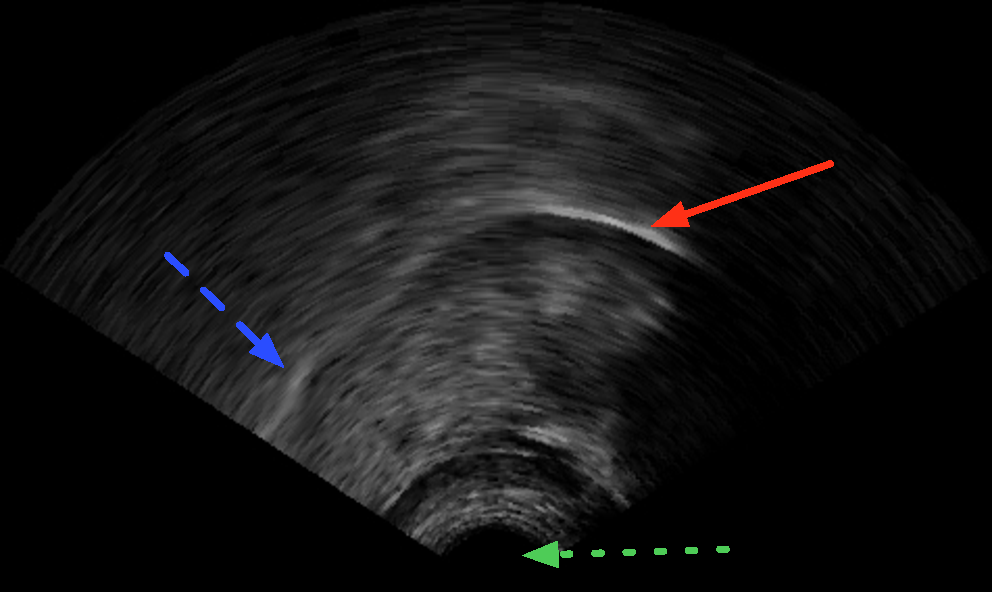
\includegraphics[width=.8\textwidth]{P2_lemon_1st_frame_annotated.pdf}
}


\frame{\frametitle{Yleistä II}
  \vspace*{-2cm}
  \hspace*{6cm}
  
\includegraphics[width=4cm]{batman}
  \vspace{.5cm}
  \begin{itemize}
  \item Lääketieteellisessä ultraäänikuvantamisessa antureilla ja
    niiden erilaisilla ominaisuuksilla on tärkeä rooli.
  \item Ne ovat lähetin-vastaanottimia -- kaikuluotaimia, jotka sekä tuottavat
    että havaitsevat ultraääntä pietsosähköisten kiteiden avulla.
  \item Laitteiden käyttämä ultraääni on hyvin korkeataajuista: 2-12 MHz
    (1 MHz = 1000 kHz = 1 miljoona Hz, vrt. ihmisen kuulon yläraja 20 kHz).
  \end{itemize}
  \centering
  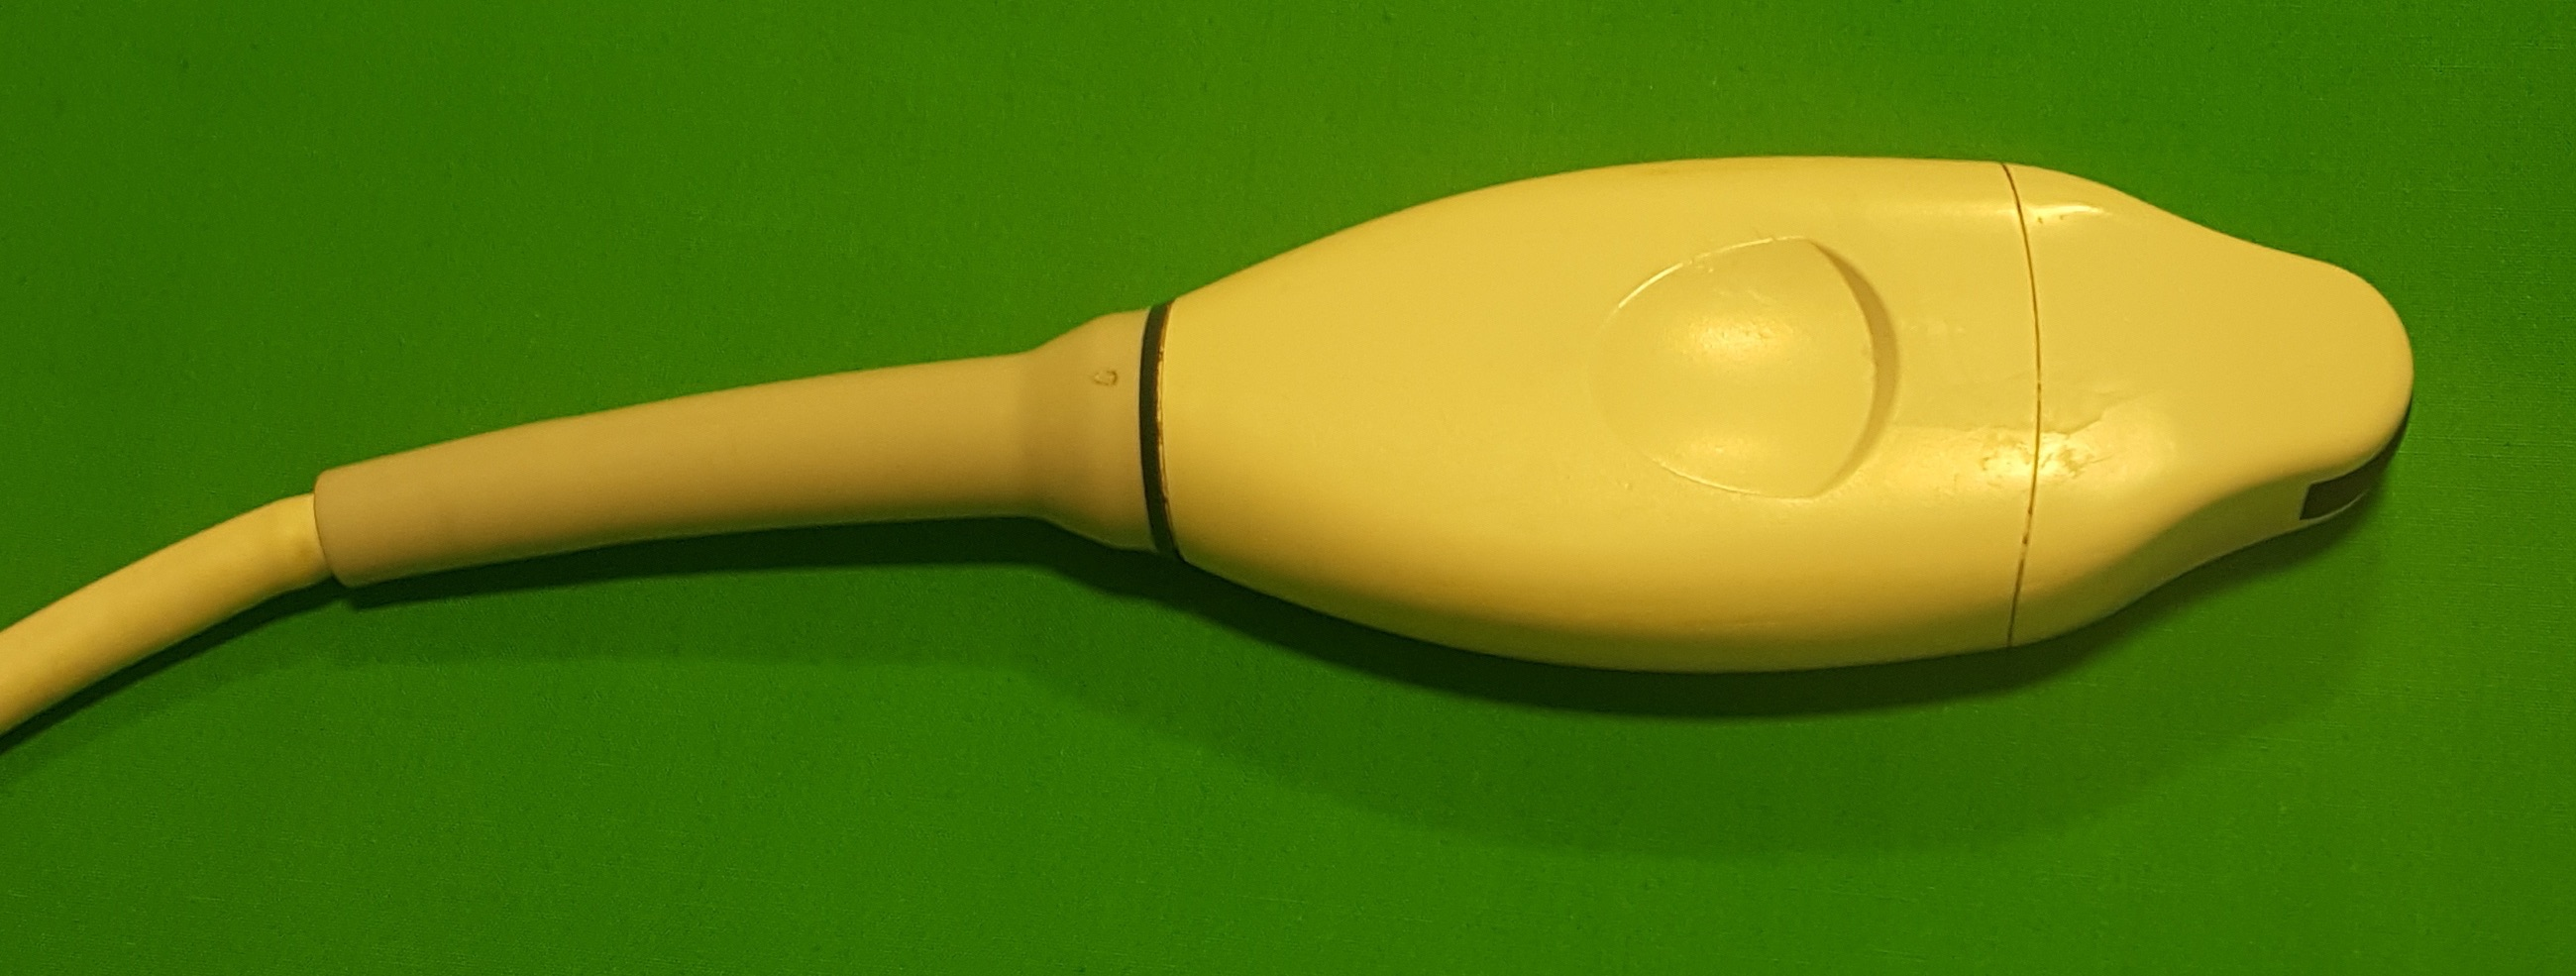
\includegraphics[height=.4\textheight]{probe.jpg}
}

\frame{\frametitle{Fyysinen toimintaperiaate}
  \begin{itemize}
  \item Ultraääniaallot kulkevat pehmeän kudoksen läpi ja heijastuvat
    takaisin erilaisista rajapinnoista.
  \item Voimakkainta heijastus on kun väliaineen äänennopeus nousee 
    tai laskee jyrkästi - kieltä kuvantaessa: 
    \begin{itemize}
      \item Voimakas heijastus kielikudoksen ja 
        ilman rajapinnasta suussa.  
      \item Lähellä anturia olevat luut näkyvät mustina varjoina
        kuvassa, koska niiden sisään ei pääse akustista energiaa (ultraääntä), 
        joten niiden sisältä ei palaa kaikuja anturin kuultavaksi.
    \end{itemize} 
  \end{itemize}
  \centering
  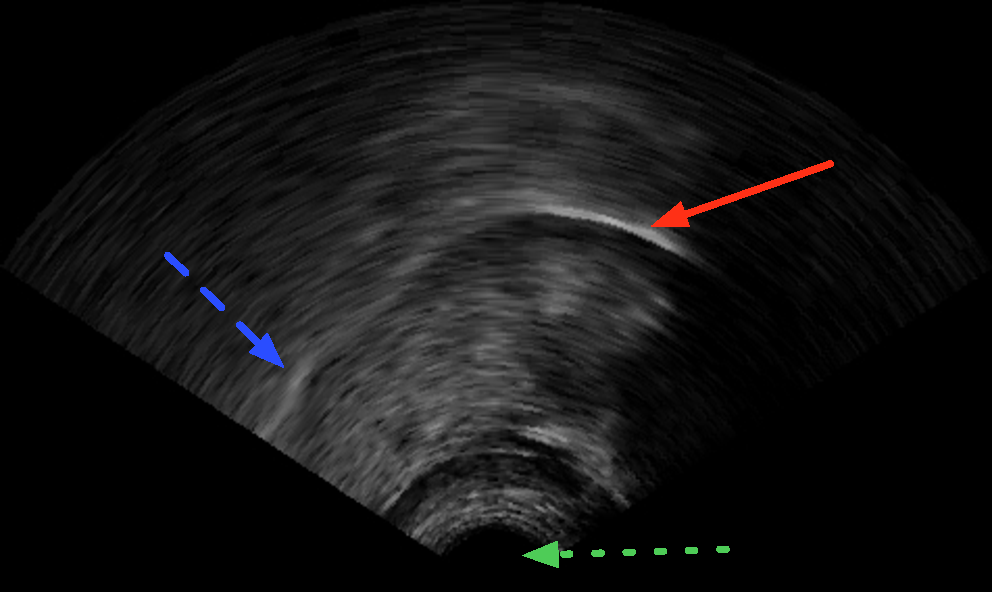
\includegraphics[width=.55\textwidth]{P2_lemon_1st_frame_annotated.pdf}
}

\frame{\frametitle{Miltä kuva näyttää? I}
  \centering
  \vfill
  Tavallinen -- kohtuu selkeä -- ultraäänikuva kielestä
  \vfill
  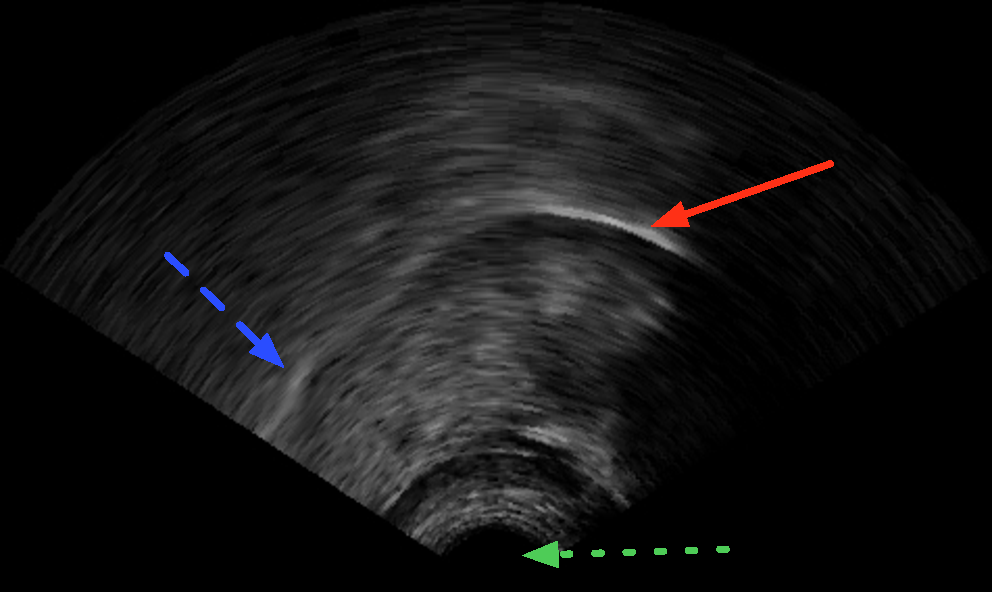
\includegraphics[width=\textwidth]{P2_lemon_1st_frame_annotated.pdf}
}

\frame{\frametitle{Miltä kuva näyttää? II}
  \centering
  \vfill
  Sivupolku: MRI kuva -- ei siis ultraäänikuva
  \vfill
  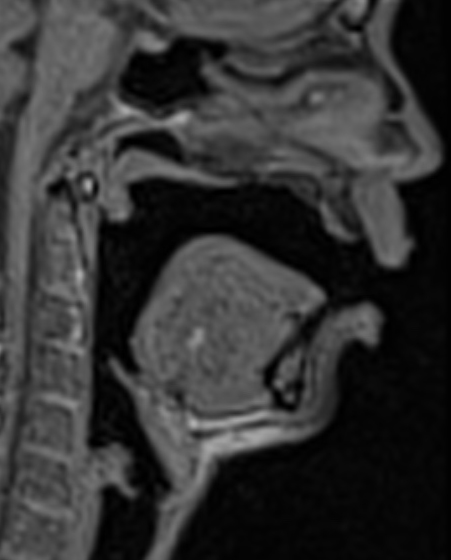
\includegraphics[height=.7\textheight]{DA_oe_cropped.jpg}
}

\frame{\frametitle{Miltä kuva näyttää? III}
  \centering
  \vfill
  Sivupolku: MRI kuvasta erotetut kudosääriviivat ja arvaamalla
  lisätyt hampaat
  \vfill
  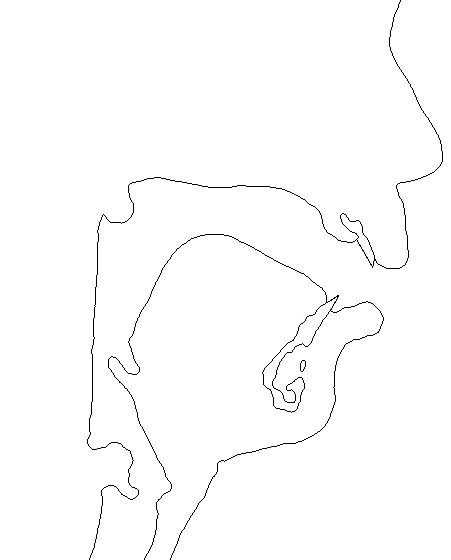
\includegraphics[height=.7\textheight]{DA_oe_hampaat_lisatty.jpg}
}

\frame{\frametitle{Miltä kuva näyttää? IV}
  \centering
  \vfill
  Kierretyn ultraäänikuvan päälle lisätty MRI:stä saatu anatomia
  \vfill
  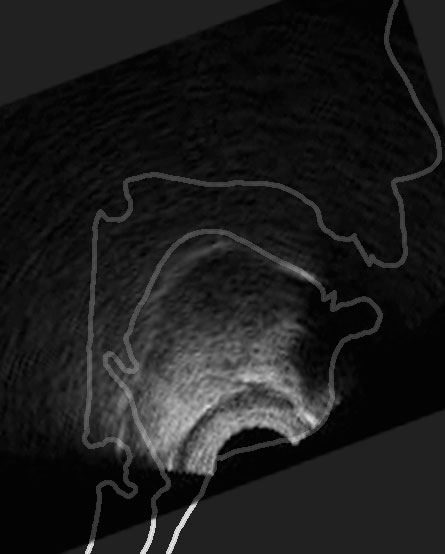
\includegraphics[height=.7\textheight]{DA_and_P1_overlay.jpg}
}

\frame{\frametitle{Miltä kuva näyttää? V}
  \centering
  \vfill
  Ultraäänikuva 'oikeassa' asennossa.\\
  (Ei tosin sama kuva kuin aiemmin.)
  \vfill
  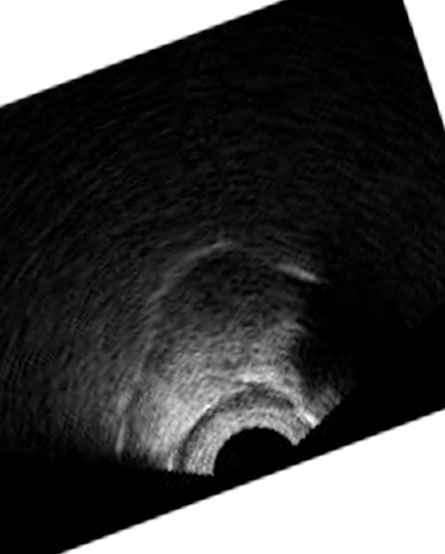
\includegraphics[height=.7\textheight]{DA_and_P1_overlay_3.jpg}
}

\frame{\frametitle{Tallennussession vaiheet}
  \begin{itemize}
  \item Puhdista kaikki.
    \begin{itemize}
    \item Laite on lääketieteellinen koje ja ihmiset ovat likaisia (ja
      korona tappaa).
    \item Aloita pesemällä ja desinfioimalla omat kädet.
    \end{itemize}
  \item Kerro osallistujalle/asiakkaalle kuinka tutkimus etenee, hoida paperihommat, näytä heille kuinka kaikki toimii.
  \item Sovita kypärä osallistujalle päähän, jos kypärä on käytössä.
  \item Tallenna data.
  \item Kerro osallistujalle, että hänestä on ollut paljon apua ja
    auta häneltä kypärä päästä.
  \item Muista antaa käsipyyhkeitä sinisen töhnän poistamiseen
    leuasta.
  \item Puhdista kaikki.
  \end{itemize}
}

\frame{
  \centering
  {
    \vfill
    \bf \Large 
    \usebeamercolor[fg]{title}
    Lyhyt tauko (5 min)
    \vfill
  }
}

\frame{
  \centering
  {
    \vfill
    \bf \Large 
    \usebeamercolor[fg]{title}
    Puheartikulaation mittaaminen ultraäänellä
    \vfill
  }
}

\frame{\frametitle{Mitä tuleman pitää - jälkimmäinen puolisko}
  \begin{itemize}
  \item Video ultraäänen käytöstä puheterapiassa
  \item Ultraäänikuvauksen toimintaperiaate ja käytännön ominaisuudet 
    \begin{itemize}
    \item Etuja
    \item Rajoitteita: Menetelmä ja ihmiset
    \item {\usebeamercolor[orange]{} \bf Kysellään}
    \end{itemize}
  \end{itemize}
}

\frame{\frametitle{Video ultraäänen käytöstä puheterapiassa}
  \begin{itemize}
    \item Amerikan englannnin puhujille 'normaalius' on sosiaalisesti hyvin
    tärkeää.
    \item Siellä(kin) /r/ on vaikea äänne ja siksi sen kuntouttamiseen nähdään
    paljon vaivaa.
    \item Video on julkaisusta: \linebreak Preston, J. L., McAllister Byun, T., Boyce, S.
    E., Hamilton, S., Tiede, M., Phillips, E., Rivera-Campos, A., \& Whalen, D.
    H. (2017). Ultrasound Images of the Tongue: A Tutorial for Assessment and
    Remediation of Speech Sound Errors. Journal of visualized experiments :
    JoVE, (119), 55123. https://doi.org/10.3791/55123
  \end{itemize}
}

\frame{\frametitle{Etuja I}
  \begin{itemize}
  \item Ultraäänikuvantaminen on hyvin turvallista kun laitetta
    käytetään matalalla tehotasolla.
  \item Ei vaadi ihmeempiä osallistujilta kunhan tallennussessiot
    eivät ole pitkiä.
  \item Helppokäyttöinen -- alkuun tosin laitteiston asentaminen ja
    opetteleminen vaativat työtä.
  \item Laitteisto mahtuu lentokäsimatkatavaraan, mitä on käytetty hyväksi
    kenttätutkimuksessa.
  \item Suhteellisen halpa hankintahinta ja hyvin halvat
    käyttökustannukset.
  \end{itemize}
}

\frame{\frametitle{Etuja II}
  \begin{itemize}
  \item Hyvä aikaresoluutio: Puhekäytössä tavanomaiset laitteet
    tuottavat kuvia 20-120 Hz taajuudella (ja erityisen hyvät
    laitteet jopa 400 Hz taajudella).
  \item Paikkaresoluutiokin on hyvä, mutta monimutkaisempi suure,
    koska resoluutio ei ole vakio kuvan sisällä.
  \end{itemize}
  
  \centering
  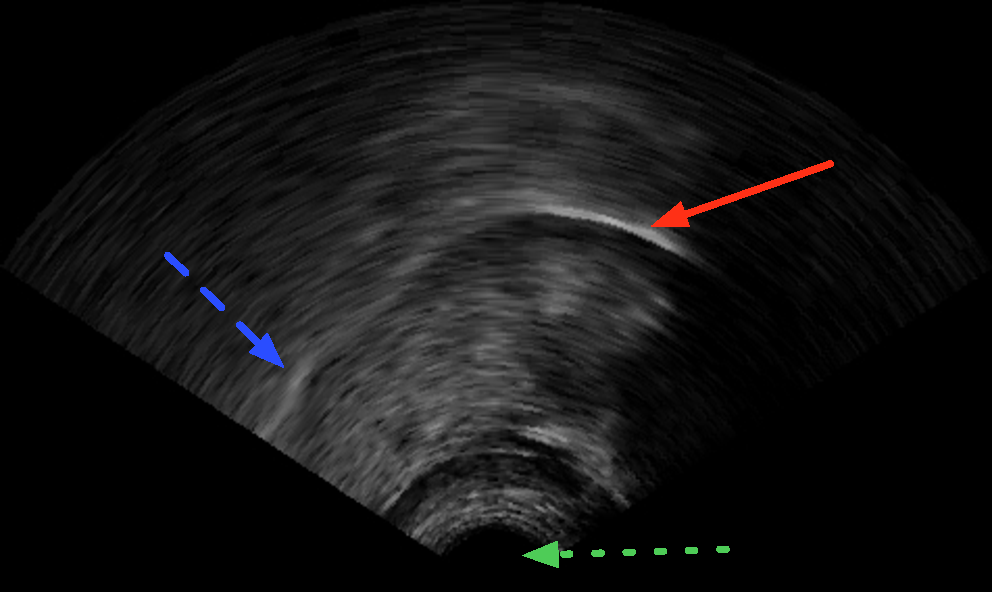
\includegraphics[width=.8\textwidth]{P2_lemon_1st_frame_annotated.pdf}
}

\frame{\frametitle{Rajoituksia I: Kuvanlaatu}
    \begin{itemize}
    \item Aikaresoluutio on kääntäen verrannollinen paikkaresoluutioon.
    \item Resoluutio ja kuvanlaatu riippuvat käytetystä ultraäänen
      taajuudesta: Matalat taajuudet läpäisevät kudokset hyvin, mutta
      tuottavat huonomman paikkaresoluution; korkeat taajuudet
      tuottavat paremman resoluution, mutta eivät läpäise kudoksia
      kovin syvälle.
    \item Erityisesti tottumattomille silmille kuvat ovat suttuisia.
    \item Suttuisuus johtuu suurelta osin kertautuvista kaiuista, kun
      ultraääniaalto heijastelee kudoksen sisällä eri rajapinnoista.
    \end{itemize}
}

\frame{\frametitle{Rajoituksia II: Mitä ylipäätään voidaan kuvata}
  \begin{itemize}
  \item Kaikkia anatomisia rakenteita ei voi kuvantaa ultraäänellä.
  \item Yleensä mistään, mikä on ilmaraon tai luun takana ei saada kuvaa.
  \item Monimutkaiset rakenteet kudosten sisällä voivat tehdä kuvien
    tulkitsemisesta hyvin vaikeaa.
  \end{itemize}
  
  \centering
  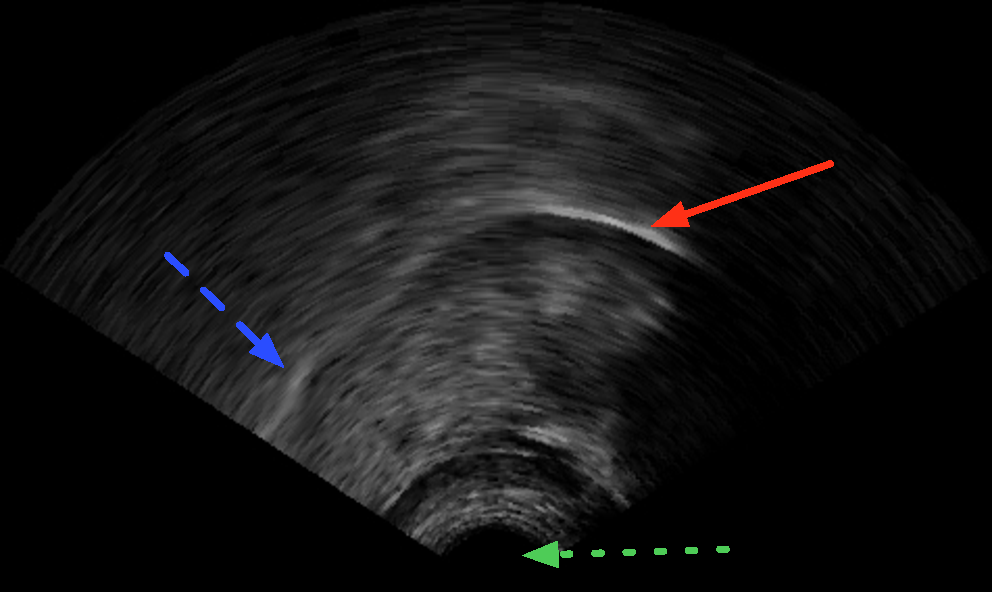
\includegraphics[width=.8\textwidth]{P2_lemon_1st_frame_annotated.pdf}
}

\frame{\frametitle{Rajoituksia III: Menetelmä ja ihmiset}
  \vfill
  Anturin vakauttamiseen käytetään erilaisia menetelmiä. Tutkimustyössä niistä
  ehkä yleisin on kypärä.
  \vfill
  \begin{columns}
    \begin{column}{.49\textwidth}
      Vanha kypärä -- painaa paljon
      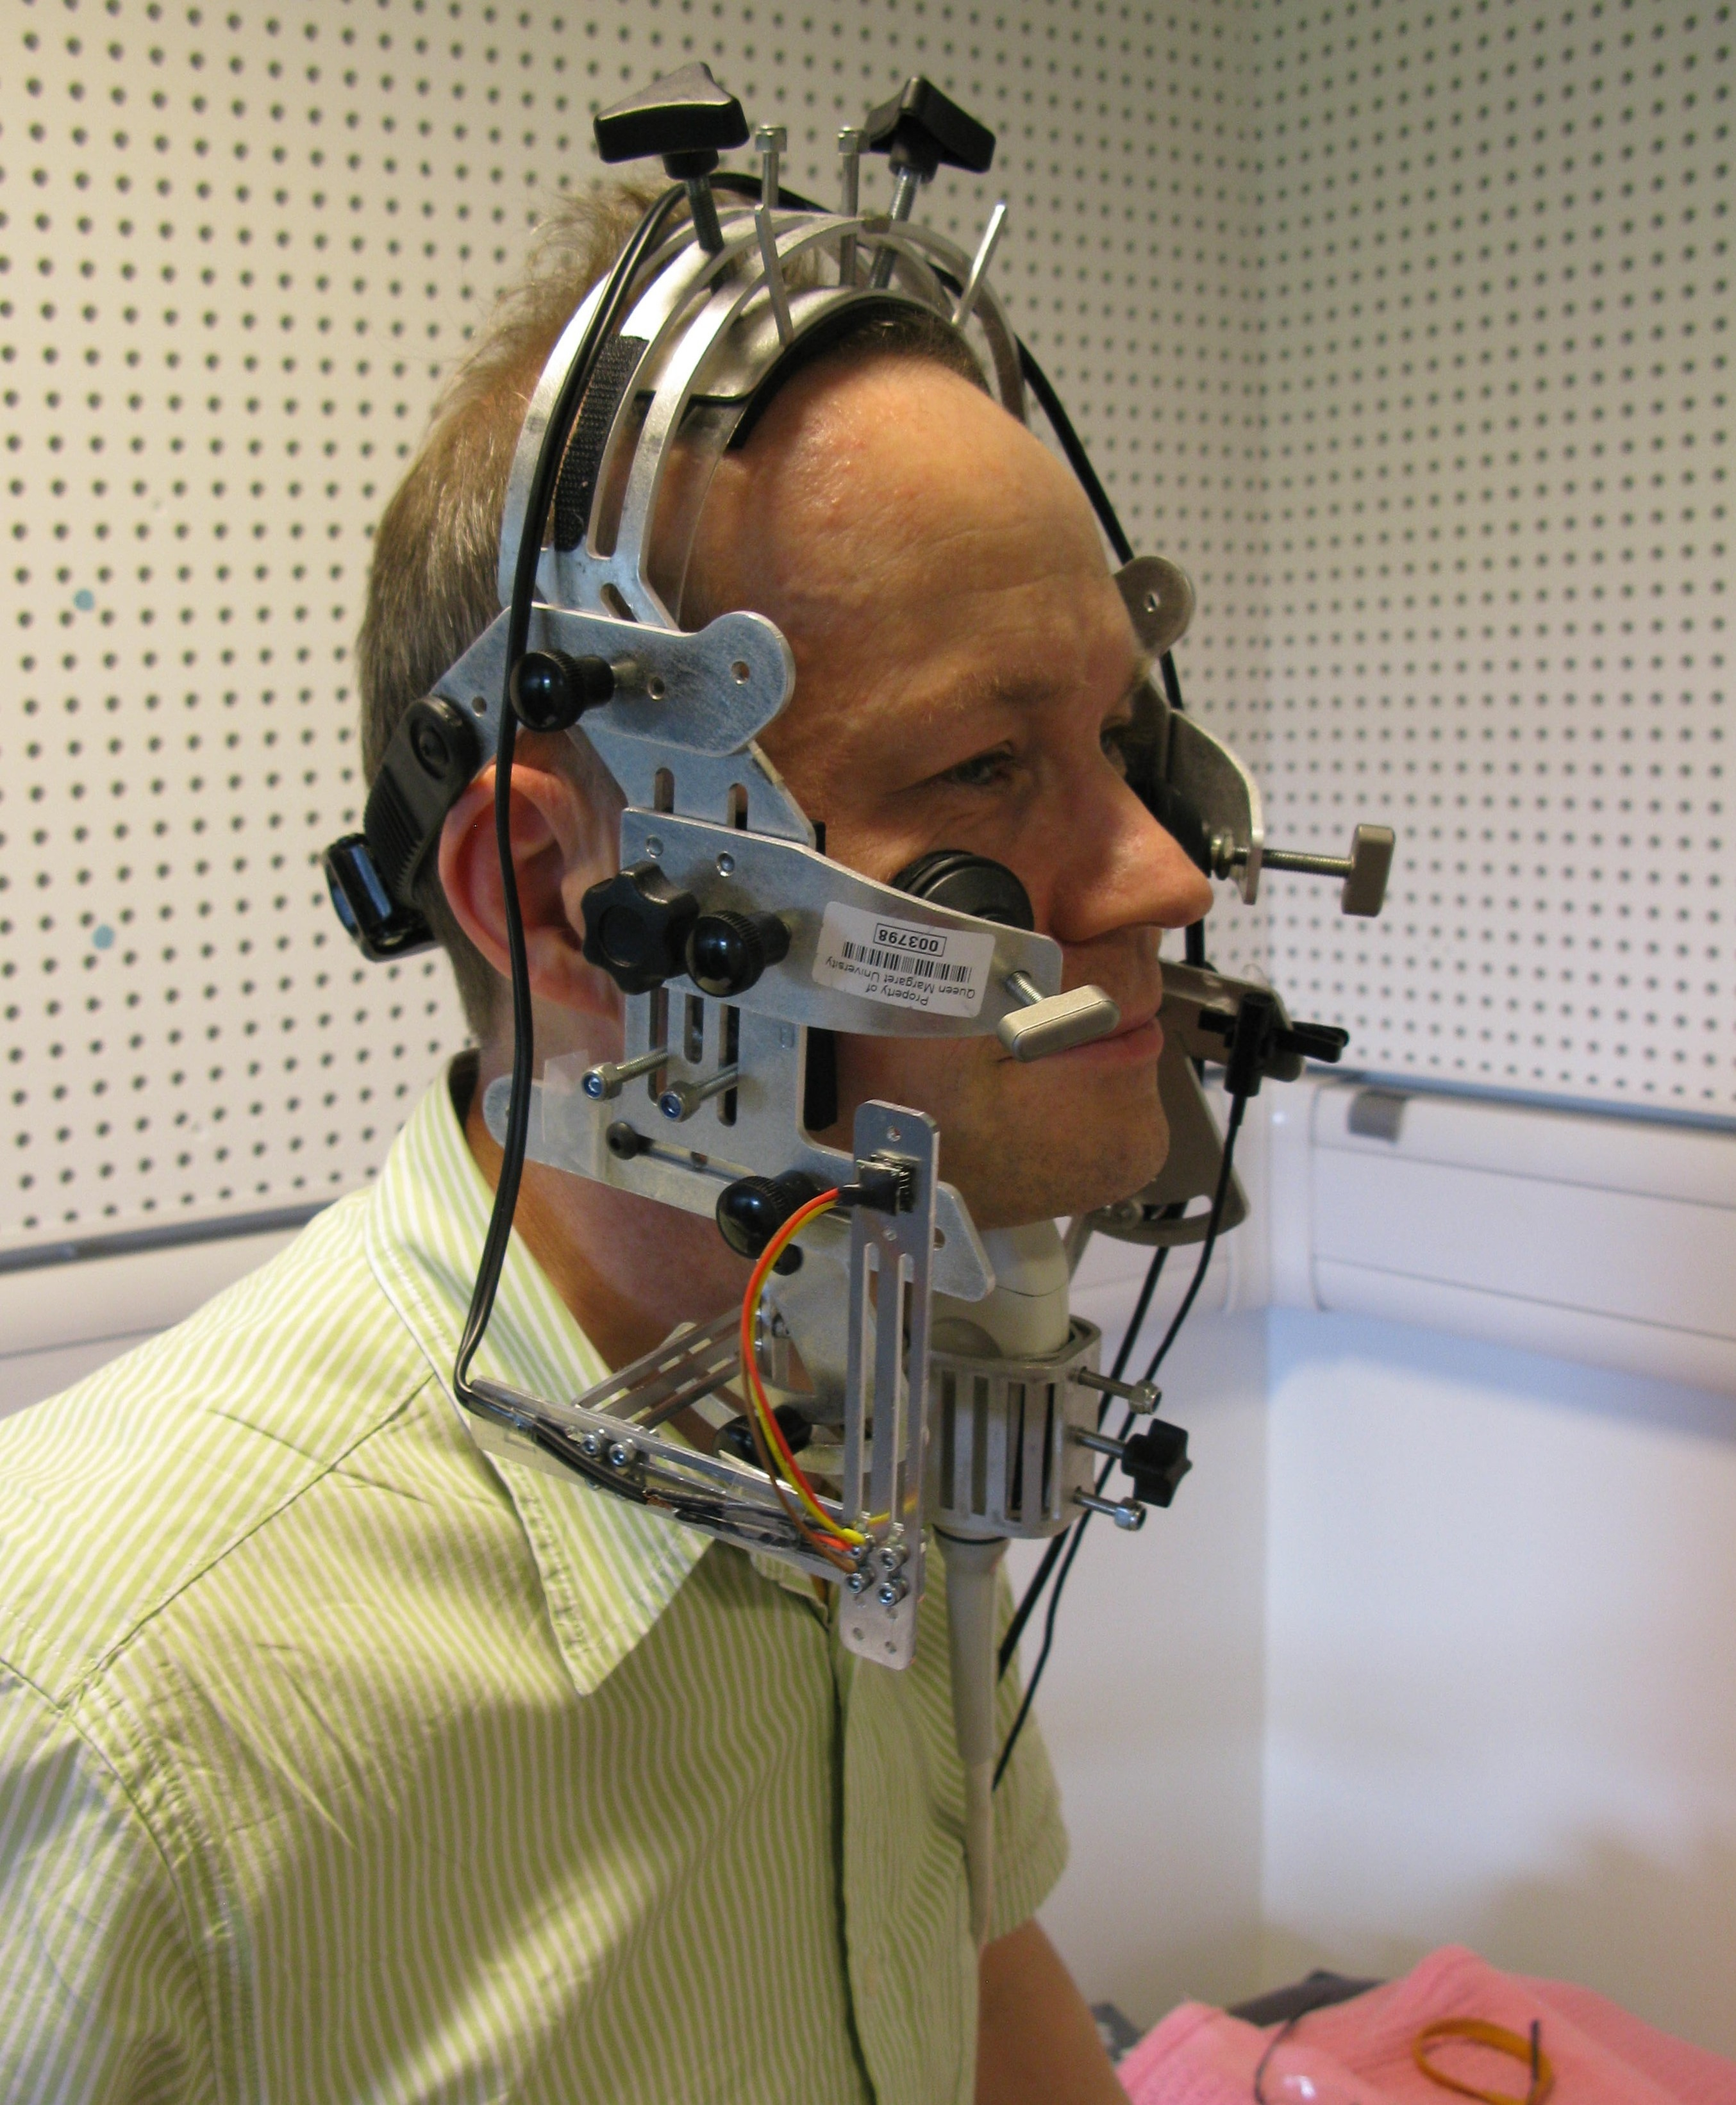
\includegraphics[width=\columnwidth]{UTI_headset.jpg}
    \end{column}
    \begin{column}{.49\textwidth}
      Uusi kypärä -- paljon kevyempi
      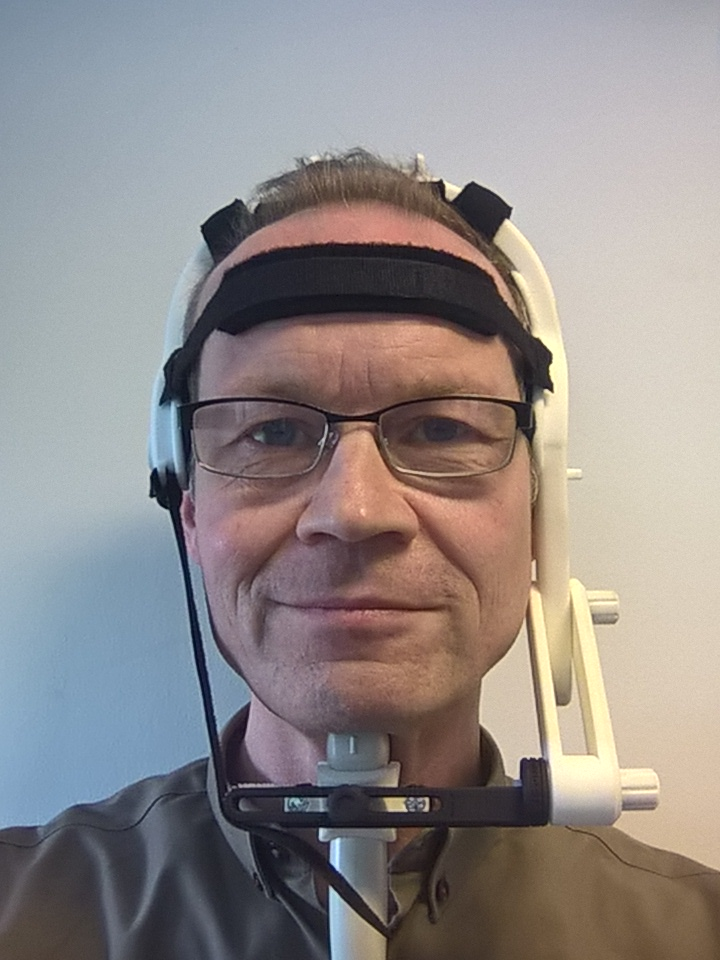
\includegraphics[width=\columnwidth]{UTI_headset_II.png}
    \end{column}
  \end{columns}  
}

\frame{\frametitle{Rajoituksia IV:  Osallistujien valinta}
  \begin{itemize}
  \item Pienet lapset eivät voi käyttää kypärää ja lapsia ylipäänsä
    on vaikea motivoida olemaan riittävän paikoillaan.
  \item Anturia voidaan pitää kädessä, mutta käsin vakautettu data
    on vaikeampaa analysoida.
  \item Suuripäiset, erityisesti suurikieliset ihmiset kuvantuvat
    huonosti.
  \item Suuri määrä rasvakudosta leuan alla tekee kuvantamisesta
    haastavaa.
  \item Ikä lisää kiinnikkeiden määrää mm. kielen
    sisällä. Kiinnikkeet aiheuttavat suttua kuvassa.
  \end{itemize}
}


\frame{
  \centering
  {
    \vfill
    \bf \Large 
    \usebeamercolor[fg]{title}
    Kyselkää
    \vfill
  }
}


\frame{\frametitle{Kirjallisuutta ja kiitokset}

  \begin{itemize}
  \item Steve Cowen: AAA:n käyttöapu ja kuva minusta.
  \item Felix Schaeffler: lepakkokuva.
  \item Alan Wrench: AAA:n käyttöapu ja laitteistokuvat.
  \item Megan Diekhoff: Kliinisen tutkimuksen vinkkit.
  \end{itemize}
  
  \bibliographystyle{apalike}
  \bibliography{bib/master}

}

\end{document}

